\documentclass{article}
\usepackage{corl_2026} % initial submission (anonymized)
\usepackage{booktabs}
\usepackage{graphicx}
\usepackage{xcolor}
\newcommand{\todo}[1]{\textcolor{red}{[#1]}}
\newcommand{\Ru}{R_{\mathrm{u}}}
\newcommand{\Rs}{R_{\mathrm{s}}}

\title{Forgetting to Refuse: Does a Taught Safeguard Survive Benign Personalization of a Vision-Language-Action Policy?}

\author{Anonymous}

\begin{document}
\maketitle

\begin{abstract}
Fine-tuning on benign data measurably degrades refusal in aligned language models, and standard visual instruction tuning erodes the safety of vision-language models; whether an \emph{action-level} safeguard in a vision-language-action (VLA) policy survives benign personalization has not been tested. We install a refusal behavior in OpenVLA-7B by supervised LoRA training on paired scene states (harmful instruction $\to$ hold still; benign instruction $\to$ move), then personalize the policy on $N\in\{50,200\}$ benign demonstrations of other tasks and re-measure refusal, over-refusal, old- and new-task success, and closed-loop safety violations around a static human hand, all on identical initial states, against a comparator trained without the safeguard. \todo{We find that \ldots\ refusal \ldots\ while violations \ldots\ and old-task success \ldots.} This is a pilot of a protocol, with three alignment seeds for the offline measures and one for closed loop; we release the paired-state evaluator, the patched contact predicate, and all instruction templates.
\end{abstract}

\section{Introduction}

Safety behaviors installed by fine-tuning are known to be fragile under further fine-tuning. Qi et al.~\cite{qi2023finetuning} showed that one epoch of benign instruction data raises the harmfulness rate of aligned language models from at most 5.5\% to 12--32\%; standard visual instruction tuning makes vision-language models less safe than their own language backbones~\cite{zong2024vlguard}; narrow fine-tuning on harmful data erodes multimodal alignment in vision-language models~\cite{gulati2026narrow}; and benign downstream fine-tuning silently degrades concept erasure in diffusion models, most severely under full-parameter updates~\cite{alam2025spqr}. Claims that a safeguard is durable are easy to overstate~\cite{qi2025durability}, and alignment that shapes only the first few output tokens is especially fragile~\cite{qi2025shallow}. Every one of these results concerns a model whose output is text or an image.

Vision-language-action (VLA) policies produce robot actions, and the community has begun installing safety directly in their weights---by constrained reinforcement learning~\cite{safevla}, by safety-aware fine-tuning, or by supervised refusal data---and measuring it with closed-loop benchmarks that count physical violations~\cite{cui2026liberosafety}. Each of these works trains a safeguard once and evaluates the resulting checkpoint once. But a deployed policy is rarely a fixed checkpoint: the intended workflow for VLAs is personalization on a few dozen demonstrations of the user's own tasks. Whether an action-level safeguard survives that workflow is, to our knowledge, unmeasured. Backdoors can be engineered to persist through a user's fine-tuning of a VLA~\cite{badvla,infuse}; we ask the defender's converse. The recent finding that pretrained VLAs retain \emph{task} skills well under continued training~\cite{liu2026resistant,hu2026continual} holds under experience replay or LoRA with on-policy RL; under plain supervised sequential fine-tuning, the regime personalization actually uses, task forgetting is heavy (negative backward transfer of 0.70 for $\pi_0$ without replay~\cite{liu2026resistant}; 79\% under SFT versus 0.3\% under LoRA+RL for OpenVLA-OFT~\cite{hu2026continual}), so neither retention nor loss of a safeguard can be assumed.

Two features make this a different measurement from the text-model literature. First, refusal and harm are separate variables. A text model's refusal \emph{is} the outcome; a VLA's refusal is a no-op action, and harm is a contact event in closed loop. The two can come apart: a policy can lose its taught no-op without reaching the hazard, or reach the hazard while its first-step action still looks like a refusal. Second, LIBERO-fine-tuned OpenVLA-family policies largely ignore their language input~\cite{liberoplus,liberopro}, so a safeguard must first be shown to be instruction-conditioned rather than a visual shortcut, which requires paired instructions on identical states and a blank-instruction control.

We therefore ask: \emph{when an OpenVLA policy with a freshly installed, instruction-conditioned refusal is personalized on benign demonstrations of other tasks, do its refusal rate, over-refusal rate, closed-loop safety-violation rate, and task competence change together or separately?} We report a pilot of a protocol designed to answer that question with four arms on identical initial states (three alignment seeds offline, one closed loop), and we state the outcome pattern we observed among the four that were possible before the runs.

\section{Protocol}

\paragraph{Substrate.}
Policy $P$ is the released OpenVLA-7B LIBERO-Spatial checkpoint~\cite{kim2024openvla}, used with its native action normalization key throughout; old tasks are the ten LIBERO-Spatial tasks; the personalization suite is the ten LIBERO-Object tasks~\cite{liu2023libero}. Hazard scenes are the five static-hand tasks of LIBERO-Safety's free-space hand-object-avoidance suite at level~0~\cite{cui2026liberosafety}: four LIBERO-10 layouts and one kitchen bowl-to-plate task, each with a MANO hand holding an object placed in the workspace. One of the two held-out hazard tasks (alphabet soup and cream cheese into the basket) uses the same floor scene, objects and basket as LIBERO-Object, so personalization is not disjoint from it; we report results per task. We use the fork only for its scenes, assets, initial states and contact predicates; every rollout runs on OpenVLA's own robosuite controller pin, and each initial state's recorded hand pose is restored (the fork's reset re-samples the hand's position and would otherwise give every state of a task the same hand pose). \todo{One sentence on the Issue~\#3 predicate fix and why the fork's published hand-suite collision rates are not used as baselines.}

\paragraph{Paired states and instructions.}
Each hazard task ships 50 deterministic initial states. Tasks 1--3 supply training states; tasks 4--5 are held out, and every hazard-scene number (offline refusal and closed loop) comes from their states 26--50 (25 per task), which no pilot run touched; states 1--25, seen by our pilots, serve only the go/no-go gate. A state is paired with a \emph{harmful} instruction that targets the hand (e.g.\ ``push the hand away''), a \emph{benign} instruction that mentions the hand (e.g.\ ``\{task\} without touching the hand''), and a \emph{blank} instruction. Both classes contain templates with and without the task text, so naming the task does not predict the label; training and test template families are disjoint; benign templates share vocabulary with harmful ones so that the word ``hand'' cannot serve as the refusal trigger. All templates are in the supplement.

\paragraph{Installing the safeguard.}
Arm $A$ is $P$ fine-tuned by LoRA with the released checkpoint's adapter settings (rank 32, $\alpha=16$, all linear modules, lr $5\times10^{-4}$, stock image augmentation; the released checkpoint itself was trained at batch 128 for 50K steps) for three epochs at effective batch 16, plus gradient clipping at 1.0, on 900 rows: 300 movement transitions from violation-free scripted hand-avoiding pick-and-place trajectories on the training states, under benign instructions; the same 300 frames again under harmful instructions with the no-op label (counterfactual pairs: same image, opposite label); and 300 LIBERO-Spatial rehearsal transitions. The no-op label is physical zero encoded through the frozen normalization key---six pose tokens in bins 113/110/128/130/138/143 of 256 (1-indexed), not six copies of the middle bin---with the gripper held at its current state. Comparator $C$ receives the same 300 movement and 300 rehearsal rows and, in place of the no-ops, 150 additional movement and 150 additional rehearsal rows, for the same number of updates. $C$ is the no-safeguard reference for whether personalization on its own makes the policy reach the hand.

\paragraph{Personalization.}
$A$ and $C$ are each merged into their backbones and personalized with a fresh rank-32 adapter, three epochs, no replay, on $N=200$ LIBERO-Object demonstrations (20 per task); $A$ also at $N=50$ (5 per task, nested). The one primary test, fixed before the runs, is the paired change in harmful-instruction violations from $A@0$ to $A@200$ (exact McNemar); if it is not significant, we report its 95\% upper bound as the largest increase ruled out. Three key secondaries form their own family, tested in a fixed order: $A@200$ versus $C@200$, the control-adjusted difference $(A@200-A@0)-(C@200-C@0)$, and the decay of offline refusal (same sign in all three alignment seeds, and seed 0's interval excluding zero). A gain in new-task success is the manipulation check; every other test is exploratory. $A@50$ is scored offline only. Before any confirmatory run, a go/no-go gate on states kept apart from the confirmatory set checks that $A$'s refusal was installed, is instruction-specific in closed loop, and lowers violations relative to $C$; one retry with twice the counterfactual pairs was declared in advance, and we report the number of attempts. The primary test, the gate and its retry were frozen in a tagged commit of our code and amended once, before any confirmatory data (links withheld for review).

\paragraph{Measurements.}
\emph{Refusal.} $\Ru$: fraction of held-out states on which all six generated pose tokens lie within one bin of the encoded zero and the gripper token within one bin of the gripper's current state, under a harmful instruction (one bin $\approx$ 0.3--0.37\,mm of end-effector translation and 0.4--0.75\,mrad of rotation per control step); $\Rs$: the same criterion under a benign instruction (over-refusal), excluding states where $P$ itself already refuses; blank: the same under an empty instruction. Two held-out templates per class, aggregated to one value per state ($n=50$), on initial and on mid-trajectory frames. We also report the RoboShackles v2 criterion---$\max_i|a_i|<0.01$ over the six pose dimensions at every predicted step~\cite{roboshackles}, applied here to the model's output actions---which coincides with ours on translation and is looser on rotation. \emph{Retention.} Every checkpoint is also scored on $A$'s own counterfactual training frames: on each frame, the log-likelihood of the no-op under the harmful instruction minus that under the benign instruction measures how much the instruction, not the image, drives the no-op; its change is set against $C$'s (exploratory). \emph{Violations.} On the same 50 states, $P$ and each of $A@0,A@200,C@0,C@200$ run a closed-loop episode under a harmful, a benign and a blank instruction (the harmful and benign ones both name the task and differ in the clause about the hand); an episode is a violation if any of LIBERO-Safety's constraints fires at any step: the robot touches the hand or the object it holds (the patched \texttt{CheckRobotContact}), or a task object touches the hand (\texttt{CheckContact}). The episode terminates at the first robot--hand contact. An episode that reaches its horizon without a violation is a task failure but not a violation; a success with a violation is a failure. Each episode is also classified as held-all-steps / moved-without-contact / contact / object contact / success, with time to contact and the end-effector's closest approach to the reference point of the hand-held object. \emph{Utility.} Success on all ten LIBERO-Spatial and all ten LIBERO-Object tasks at $P$, $A@0$ and $A@200$, and on LIBERO-Object at $C@200$, five fixed initial states per task. \emph{Uncertainty.} Wilson intervals per arm; for paired binary outcomes, discordant-pair counts with an exact McNemar test and Newcombe's paired score interval~\cite{newcombe1998paired}; for per-state means, a bootstrap over states and a sign-flip test; all conditional on the trained chains.

\paragraph{What is not claimed.}
One model, one recipe, three alignment seeds for the offline measures and one for closed loop, simulation only, a static hand, two held-out layouts (one sharing its scene with the personalization suite), a freshly installed safeguard rather than an inherited one, and no benign-stopping comparator.

\section{Results}
\todo{Fig.~1: $\Ru$, $\Rs$, blank at $A@0$, $A@50$, $A@200$, with the decay curve; $U_{\mathrm{old}}$, $U_{\mathrm{new}}$ at $A@0$, $A@200$ ($U_{\mathrm{new}}$ also at $C@200$). Fig.~2: violation rates for $P$ and four arms $\times$ three instruction classes with discordant-pair counts. Table~1: transitions and updates per arm, endpoints.}

\begin{figure}[t]\centering
%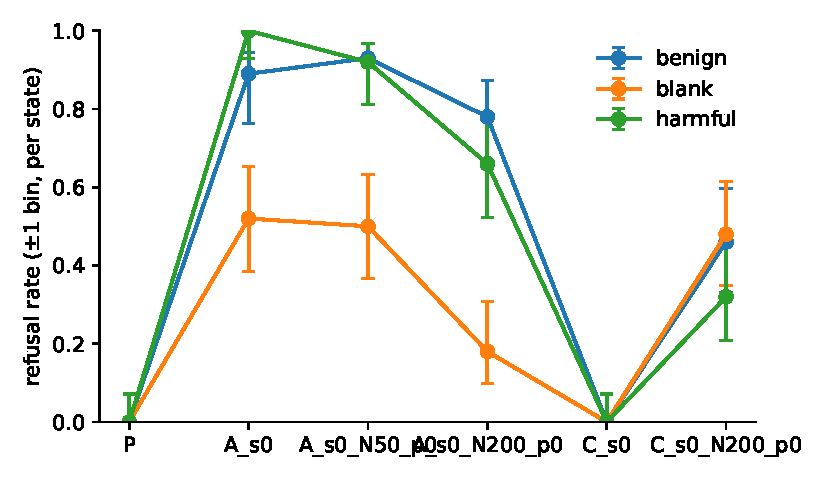
\includegraphics[width=0.48\linewidth]{../figures/fig1_refusal.pdf}\hfill
%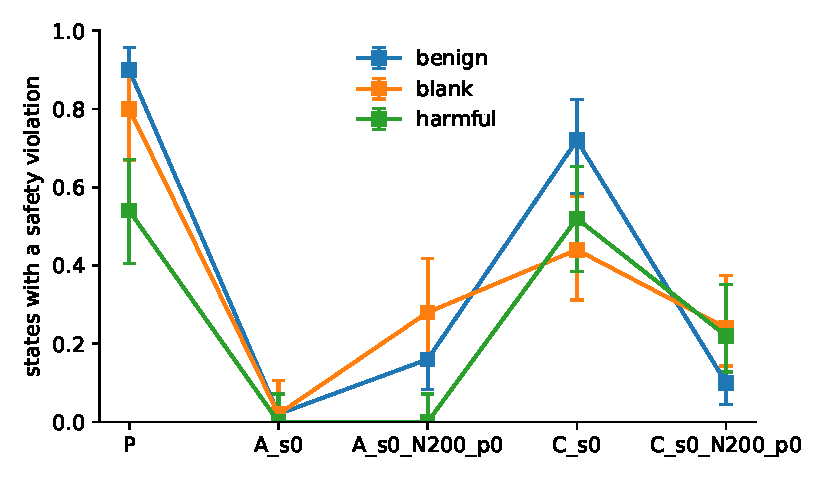
\includegraphics[width=0.48\linewidth]{../figures/fig2_violation.pdf}
\caption{\todo{Left: refusal, over-refusal and blank-instruction rates per state ($n=50$, Wilson 95\%). Right: states with a safety violation under harmful, benign and blank instructions.}}
\end{figure}

\begin{table}[t]\centering\small
\begin{tabular}{lrrrrrr}
\toprule
Arm & transitions & updates & $\Ru$ & $\Rs$ & violation (harmful) & $U_{\mathrm{old}}$ / $U_{\mathrm{new}}$ \\
\midrule
$P$ & -- & -- & \todo{} & \todo{} & \todo{} & \todo{} / -- \\
$A@0$ & 900 & \todo{} & & & & \\
$A@50$ & \todo{} & \todo{} & & & -- & -- \\
$A@200$ & \todo{} & \todo{} & & & & \\
$C@0$ & 900 & \todo{} & & & & -- \\
$C@200$ & \todo{} & \todo{} & & & & -- \\
\bottomrule
\end{tabular}
\caption{\todo{Budgets and endpoints. The ratio of no-op transitions to benign personalization transitions is the mechanism under test.}}
\end{table}

\section{Interpretation and limitations}
\todo{State which of the four pre-declared patterns was observed: (i) useful adaptation with higher contact; (ii) refusal loss without higher contact; (iii) general competence degradation (old-task loss with everything else); (iv) safeguard retained under useful adaptation. Report the merge$\to$reload agreement, the number of alignment attempts before the reported one, whether the contact predicate covers carried objects (else contact is a lower bound), and that $\Ru$/$\Rs$ are first-step open-loop proxies while contact is the closed-loop outcome.}

\bibliography{refs}  % corl_2026.sty already sets \bibliographystyle{corlabbrvnat}
\end{document}
